\documentclass[11pt,a4paper]{article}

\usepackage[utf8]{inputenc}
\usepackage[T1]{fontenc}
\usepackage{hyperref}
\usepackage{url}
\usepackage{booktabs}
\usepackage{graphicx}
\usepackage{listings}
\usepackage{xcolor}
\usepackage{amsmath}

\usepackage{geometry}
\geometry{margin=1in}

\lstset{
  basicstyle=\ttfamily\small,
  breaklines=true,
  frame=single,
  backgroundcolor=\color{gray!8},
  commentstyle=\color{gray},
  keywordstyle=\color{blue!70},
}

\title{\textbf{skillgraph-mcp}: Progressive Disclosure and Semantic Skill Graphs\\
       for Multi-Server MCP Deployments}

\author{
  Javier Rodeiro Rodr\'iguez \\
  \href{https://github.com/jrodeiro5/skillgraph-mcp}{github.com/jrodeiro5/skillgraph-mcp}
}

\date{May 2026}

\begin{document}

\maketitle

\begin{abstract}
As AI agents connect to increasing numbers of Model Context Protocol (MCP) servers,
tool proliferation degrades agent performance. An agent wiring ten MCP servers may
receive over 100 tool schemas in its context window before any user message is
processed---a phenomenon we term \emph{tool bloat}. We present \textbf{skillgraph-mcp},
an open-source MCP gateway built on top of skillful-mcp~\cite{skillful2026} that addresses
tool bloat through two mechanisms: (1)~\emph{progressive disclosure}, where the agent sees
a compact skill index upfront and retrieves per-server schemas on demand, and
(2)~a \emph{semantic skill graph} encoding prerequisite and successor relationships
between tools, enabling structured workflow planning. In a deployment of ten downstream
servers exposing 113~tools, skillgraph-mcp reduces upfront context consumption from
approximately 3,660~tokens to 287~tokens---a \textbf{92\% reduction}---while preserving
full tool access. The gateway becomes beneficial at four or more servers (approximately
nine tools); below this threshold the gateway overhead exceeds the schema cost it
replaces. We further describe \textbf{SkillOpt}, a background loop that uses execution
traces to continuously refine tool descriptions and graph relations via LLM feedback
without manual annotation. skillgraph-mcp is production-ready, ships prebuilt binaries
for six platforms, and is available as open source~\cite{skillgraph2026}.
\end{abstract}

%──────────────────────────────────────────────────────────────────────────────
\section{Introduction}
\label{sec:intro}

The Model Context Protocol~\cite{mcp2024} has rapidly become the standard integration
layer between AI agents and external capabilities. An agent developer today may connect
10--20 MCP servers---search, memory, browser automation, code intelligence,
databases---each exposing anywhere from 1 to 30+ tools.

This creates a structural problem: MCP clients load all registered server schemas at
connection time. Every tool's name, description, and JSON Schema \texttt{inputSchema}
enters the model's context window before the user types a single word. With ten servers
and 113~tools, this pre-task overhead reaches approximately 3,660~tokens. At
20~servers, it approaches 7,000~tokens---a significant fraction of the effective
working context, consumed by capability declarations rather than task-relevant content.

We observe that most agent tasks use a small subset of available tools. A user asking
``search for papers on attention mechanisms'' needs brave-search or firecrawl---not
Playwright, gitnexus, wsl-terminal, or postgres. Yet all of their schemas are loaded
regardless.

This paper presents skillgraph-mcp, a gateway that applies \emph{progressive
disclosure} to MCP tool loading. The agent sees a 10-line skill index upfront and
requests per-server schemas only when needed. We report empirical measurements of the
token savings, characterize when the gateway is and is not beneficial, describe the
semantic skill graph that guides tool selection, and present SkillOpt---a trace-driven
self-improvement loop that refines the graph without annotation.

%──────────────────────────────────────────────────────────────────────────────
\section{Background and Related Work}
\label{sec:related}

\paragraph{Tool bloat in MCP deployments.}
Tool bloat was first described by Van Gent~\cite{vangent2026blog} in the context of
skillful-mcp~\cite{skillful2026}, the upstream project this work builds on. Van Gent
observed that context consumption grows linearly with registered servers and proposed a
gateway architecture with eight fixed discovery tools as the solution. skillgraph-mcp
extends this with a semantic graph structure and the SkillOpt loop.

\paragraph{Enterprise MCP gateways.}
Microsoft MCP Gateway~\cite{msgwateway2025} addresses the operational concerns of
multi-server deployments: Kubernetes lifecycle, RBAC, and adapter routing. These
systems solve the \emph{deployment} problem; they do not reduce agent context
consumption. skillgraph-mcp solves the \emph{cognition} problem and is complementary.

\paragraph{Client-side progressive disclosure.}
NousResearch's Hermes tool-search~\cite{hermes2025} implements progressive disclosure
at the \emph{client} layer: three bridge tools replace all tool schemas, activating
when tool context exceeds 10\% of the context budget. skillgraph-mcp implements the
same concept at the \emph{server} layer, making it transparent to the client and
compatible with any MCP client without modification.

\paragraph{Context budget management.}
Claude Code v2.1.105 introduced \texttt{skillListingBudgetFraction}~\cite{claudecode2026settings},
which limits the fraction of context reserved for skill descriptions. When exceeded,
least-used skill descriptions are collapsed to bare names. This is a client-side
graceful degradation mechanism operating on skill metadata; skillgraph-mcp provides
server-side schema hiding that prevents schemas from entering the context at all.
The two mechanisms are complementary.

%──────────────────────────────────────────────────────────────────────────────
\section{System Design}
\label{sec:design}

\subsection{Gateway Architecture}

skillgraph-mcp acts as a single MCP server to the client and a multi-server client
to $N$ downstream MCP servers. It exposes exactly eight gateway tools regardless of
how many downstream servers are connected (Table~\ref{tab:tools}).

\begin{table}[h]
\centering
\small
\begin{tabular}{ll}
\toprule
\textbf{Tool} & \textbf{Purpose} \\
\midrule
\texttt{list\_skills}    & Compact index: skill name + one-line description \\
\texttt{use\_skill}      & Full tool schemas for one skill, on demand \\
\texttt{execute\_code}   & Python sandbox; all downstream tools callable by name \\
\texttt{plan\_workflow}  & Skill graph traversal for multi-step task planning \\
\texttt{get\_skill\_graph} & Full graph dump (nodes + edges) \\
\texttt{read\_lattice}   & Generated docs (\texttt{skills.md}, \texttt{relations.md}) \\
\texttt{read\_resource}  & Downstream MCP resources \\
\texttt{register\_server} & Runtime server registration (loopback-only) \\
\bottomrule
\end{tabular}
\caption{The eight gateway tools exposed to the agent, independent of server count.}
\label{tab:tools}
\end{table}

\subsection{Progressive Disclosure Mechanics}

At session start, the agent receives \texttt{list\_skills} output: one line per skill
with name and description ($\approx$28~tokens/skill at 10~skills $=$ 287~tokens
total). To use a specific server, the agent calls \texttt{use\_skill(skill\_name)} and
receives that server's full tool schemas ($\approx$32~tokens/tool empirically). Unused
servers cost zero additional tokens beyond their single listing entry.

The crossover point---where gateway overhead equals raw schema cost---occurs at
approximately four servers ($\approx$9~tools). Below this threshold, deploying the
gateway increases rather than decreases context consumption.

\subsection{Semantic Skill Graph}

An in-memory directed graph (3~node types: Skill, Tool, Resource; 5~edge types:
\textsc{has\_tool}, \textsc{prerequisite\_for}, \textsc{produces}, \textsc{requires},
\textsc{common\_next\_step}) encodes relationships between tools across servers.
Example: \texttt{resolve\_library\_id} is \textsc{prerequisite\_for} \texttt{query\_docs}.
The agent calls \texttt{plan\_workflow} to retrieve a traversal over this graph for a
given task description, receiving an ordered list of tool calls to execute.

\subsection{SkillOpt: Trace-Driven Self-Improvement}

Two background goroutines run continuously:

\textbf{Bootstrap loop.} On startup, fetches GitHub READMEs for each downstream
server, sends tools and README to an LLM, and generates initial descriptions and graph
relations seeded into the configuration file.

\textbf{Refinement loop.} Polls trace files written by \texttt{execute\_code} every
30~seconds. Batches up to 10~trajectory files (code, tool calls, results, errors) and
asks the LLM to propose edits to tool descriptions and graph edges. Proposed edits are
validated (hallucinated tool names are rejected) and merged atomically via temp-file
rename, then \texttt{RebuildGraph} is called. The LLM provider is configurable;
the loop skips silently if unconfigured.

%──────────────────────────────────────────────────────────────────────────────
\section{Evaluation}
\label{sec:eval}

\subsection{Experimental Setup}

We deploy skillgraph-mcp with ten downstream MCP servers spanning 113~tools
(Table~\ref{tab:servers}). All measurements taken on a local WSL2 environment
(Ubuntu, Intel x86-64). Token estimates use 4~characters per token (conservative;
JSON Schema inputs with deeply nested objects tokenize at a higher ratio). The
per-tool token rate (32.4~tokens/tool) is empirically measured from the
\texttt{use\_skill("playwright")} response (23~tools, 2,981~characters, 745~tokens).

\begin{table}[h]
\centering
\small
\begin{tabular}{lrl}
\toprule
\textbf{Server} & \textbf{Tools} & \textbf{Category} \\
\midrule
chrome-devtools    & 29 & Browser automation \\
playwright         & 23 & Browser automation \\
firecrawl          & 20 & Web extraction \\
wsl-terminal       & 10 & Shell / SSH \\
gitnexus           & 13 & Code intelligence \\
memory             &  9 & Agent memory \\
magic              &  4 & UI generation \\
context7           &  2 & Documentation \\
brave-search       &  2 & Web search \\
sequential-thinking &  1 & Reasoning \\
\midrule
\textbf{Total}     & \textbf{113} & \\
\bottomrule
\end{tabular}
\caption{Ten downstream MCP servers in the evaluation deployment.}
\label{tab:servers}
\end{table}

\subsection{Upfront Token Cost}

Table~\ref{tab:upfront} and Figure~\ref{fig:scaling} show the primary result: a 92\%
reduction in upfront tokens consumed at session start.

\begin{table}[h]
\centering
\begin{tabular}{lrr}
\toprule
\textbf{Configuration} & \textbf{Tools} & \textbf{Tokens} \\
\midrule
Raw (all schemas loaded)      & 113 & $\approx$3,661 \\
skillgraph-mcp (\texttt{list\_skills}) & 10 skills & 287 \\
\midrule
\textbf{Reduction}            & \textbf{91\%} & \textbf{92\%} \\
\bottomrule
\end{tabular}
\caption{Upfront token cost: raw loading vs. skillgraph-mcp gateway.}
\label{tab:upfront}
\end{table}

\begin{figure}[h]
\centering
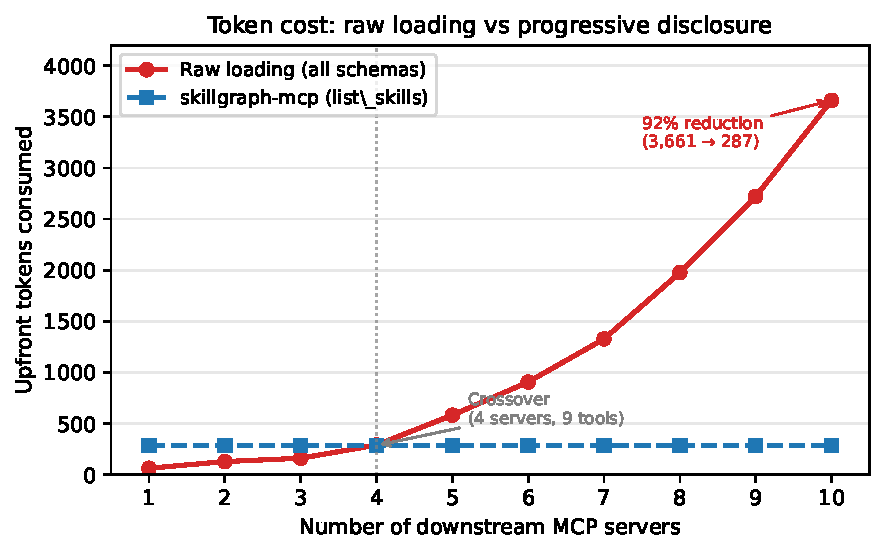
\includegraphics[width=0.82\linewidth]{figures/fig1_scaling.pdf}
\caption{Token cost as downstream servers are added (smallest to largest by tool count).
Gateway cost is constant at 287~tokens; raw cost grows linearly. Crossover at
$\approx$4~servers / 9~tools.}
\label{fig:scaling}
\end{figure}

\subsection{Per-Task Cost Model}

\begin{figure}[h]
\centering
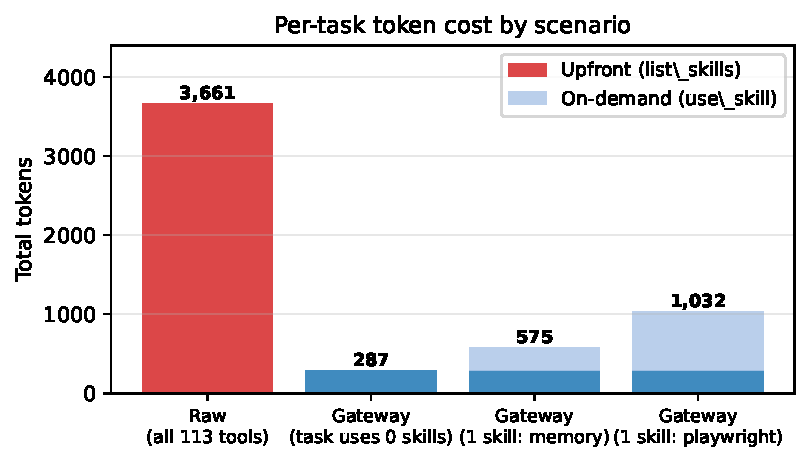
\includegraphics[width=0.75\linewidth]{figures/fig2_per_task.pdf}
\caption{Total token cost per task scenario. ``On-demand'' bars show the additional
cost of calling \texttt{use\_skill} for one server.}
\label{fig:pertask}
\end{figure}

Figure~\ref{fig:pertask} shows the per-task cost model. An agent using no
\texttt{use\_skill} calls (task solved via context alone) pays 287~tokens. An agent
activating memory (9~tools, $\approx$288~tokens) pays 575~tokens total. An agent
activating playwright (23~tools, 745~tokens) pays 1,032~tokens---versus 3,661~tokens
for raw loading. The savings increase as more servers are registered; tasks that use
only small servers benefit most.

\subsection{Demo Interaction}

The following condensed transcript captures an actual agent session through the
gateway. The agent stores research findings in persistent memory, touching only one
of ten registered servers:

\begin{lstlisting}[language=Python, caption={Agent interaction via skillgraph-mcp gateway.}]
# Step 1: Agent calls list_skills (287 tokens, all 10 servers visible)
>> list_skills()
<< brave-search, chrome-devtools, context7, firecrawl, gitnexus,
   magic, memory, playwright, sequential-thinking, wsl-terminal
   (9 servers / 104 tools never load their schemas)

# Step 2: Agent inspects memory skill (288 tokens, 9 tools revealed)
>> use_skill("memory")
<< create_entities, add_observations, search_nodes,
   create_relations, read_graph, open_nodes,
   delete_entities, delete_observations, delete_relations

# Step 3: Agent chains 3 tools in one execute_code call
>> execute_code("""
   create_entities(entities=[{
       "name": "skillgraph-mcp", "entityType": "Project",
       "observations": ["92% upfront token reduction", ...]
   }])
   create_relations(relations=[
       {"from": "skillgraph-mcp", "relationType": "extends",
        "to": "skillful-mcp"}
   ])
   graph = read_graph()
   return f"{len(graph['entities'])} entities stored"
""")
<< "3 entities, 3 relations stored"

# Total: 287 + 288 + ~150 = 725 tokens  (raw baseline: 3,661)
\end{lstlisting}

%──────────────────────────────────────────────────────────────────────────────
\section{Limitations and Future Work}
\label{sec:limitations}

\paragraph{No task accuracy measurement.}
We measure token cost reduction, not whether agents make better tool selections.
A controlled experiment comparing task success rates with and without the gateway
on standard agent benchmarks is left for future work.

\paragraph{SkillOpt not evaluated.}
The claim that SkillOpt improves routing accuracy over time is a hypothesis; no
before-and-after evaluation has been conducted.

\paragraph{Fixed per-tool token rate.}
The 32.4~tokens/tool rate is measured from a single server (Playwright). Servers
with complex nested JSON Schemas may exhibit higher rates.

\paragraph{Crossover threshold.}
Users with only a few large servers benefit earlier than the 4-server threshold
suggests. Users with 1--3 small servers should not deploy the gateway.

\paragraph{Future directions.}
Measuring task success rate on standard agent benchmarks;
evaluating SkillOpt description quality via blind human evaluation;
implicit discovery mode (transparent \texttt{use\_skill} calls);
integration with persistent trace indexing for semantic retrieval
of historically successful tool chains.

%──────────────────────────────────────────────────────────────────────────────
\section{Conclusion}
\label{sec:conclusion}

skillgraph-mcp demonstrates that a lightweight gateway layer applying progressive
disclosure to MCP tool schemas reduces agent upfront context consumption by 92\% in
a 10-server deployment, with linear improvement as server count grows. The semantic
skill graph and SkillOpt loop provide structural guidance and annotation-free
improvement without modifying the MCP protocol or downstream servers. The crossover
threshold ($\approx$4~servers, $\approx$9~tools) provides a clear decision criterion
for practitioners evaluating whether to deploy the gateway.

%──────────────────────────────────────────────────────────────────────────────
\paragraph{Acknowledgements.}
This work builds on skillful-mcp by Kurtis Van Gent (MIT License). The progressive
disclosure architecture is due to Van Gent; this paper contributes the semantic skill
graph, SkillOpt loop, CLI diagnostics, and empirical token measurements.

\bibliographystyle{plain}
\bibliography{paper}

\end{document}
